% Journal submission entry point. Scientific content is shared.
\documentclass[9pt,twocolumn,twoside]{pnas-new}
% Add the lineno option to show line numbers for review.

\articletype{APPLIED PHYSICAL SCIENCES} % TODO PNAS classification (Applied Physical Sciences or Chemistry), decide at submission
\templatetype{pnasresearcharticle}

% Initial TeX Live 2024 binaries lose \aftergroup callbacks in \output
% (https://github.com/latex3/latex2e/issues/1311). Flush any pending
% PNAS sidebar after the first column, before \Parasplit clears the page.
% With a fixed engine, the callback has already run and this is a no-op.
\makeatletter
\patchcmd{\Parasplit}{\eject\clearpage}{%
  \eject
  \ifx\AP@\relax\else
    \global\output\expandafter{\the\AP@output}%
    \global\expandafter\let\expandafter\AP@\expandafter\relax\AP@
  \fi
  \clearpage
}{}{\PackageError{pnas-firstpage}{Could not patch \string\Parasplit}{Check the PNAS template version.}}
\makeatother

% Journal-specific title, abstract, sidebar and first-page layout.
\newcommand{\NDFTMakeTitle}{%
\maketitle
\thispagestyle{firststyle}
\ifthenelse{\boolean{shortarticle}}{\ifthenelse{\boolean{singlecolumn}}{\abscontentformatted}{\abscontent}}{}

\Firstpage
}

% Shared notation and packages.
\usepackage{amsmath,amssymb,bm}
\usepackage{pifont}
\let\openbox\relax
\usepackage{amsthm}
\graphicspath{{figures/}{../figures/}}
\newcommand{\vr}{\mathbf r}
\newcommand{\vn}{\mathbf n}
\newcommand{\vz}{\mathbf z}
\newcommand{\vf}{\mathbf f}
\newcommand{\T}{\mathsf T}
\newcommand{\rmd}{\mathrm d}
\newcommand{\Fid}{F_{\rm id}}
\newcommand{\FC}{F_{\rm Coul}}
\newcommand{\Fex}{F_{\rm ex}}
\newcommand{\nb}{\bar n}
\newcommand{\methodsref}{\textit{Materials and Methods}}

\newcommand{\openingletter}[1]{#1}
\newcommand{\layoutbreak}{}
\newcommand{\siref}{\textit{Supplementary Information}}

% Shared title, author information and declarations.
\newcommand{\PaperTitle}{A structure-preserving neural density functional for the ions of a polymer electrolyte}
\newcommand{\PaperAuthor}{Liyao Lyu}
\newcommand{\PaperLeadAuthor}{Lyu}
\newcommand{\PaperAffiliationA}{School of Artificial Intelligence and Data Science, University of Science and Technology of China, Hefei, Anhui, China}
\newcommand{\PaperAffiliationB}{Suzhou Institute for Advanced Research, University of Science and Technology of China, Suzhou, Jiangsu, China}
\newcommand{\PaperAffiliationC}{Suzhou Big Data \& AI Research and Engineering Center, Suzhou, Jiangsu, China}
\newcommand{\PaperEmail}{lyuliyao@ustc.edu.cn}
\newcommand{\PaperKeywords}{classical density functional theory $|$ polymer electrolytes $|$ many-body ion correlations $|$ machine learning $|$ force matching}
\newcommand{\PaperDeclaration}{The authors declare no competing interest.}
\newcommand{\PaperAcknowledgments}{[To add.]}
\newcommand{\PaperDataAvailability}{The project repository is \url{https://github.com/Lyuliyao/NDFT_salt_doped_polymer}. It contains manuscript and figure sources, analysis and training code, model configurations, saved metrics and selected trained parameters. Raw MD trajectories and processed profiles are stored separately. [Public access, archival version and raw-data access arrangements to be confirmed before submission.]}

\renewcommand{\openingletter}[1]{\dropcap{#1}}
\renewcommand{\layoutbreak}{\Parasplit}
\renewcommand{\siref}{\textit{SI Appendix}}
\newcommand{\tablenote}[1]{\addtabletext{#1}}

\begin{document}
\title{\PaperTitle}
\hypersetup{pdfauthor={\PaperAuthor},pdftitle={\PaperTitle}}
\author[a,b,c,1]{\PaperAuthor}
\affil[a]{\PaperAffiliationA}
\affil[b]{\PaperAffiliationB}
\affil[c]{\PaperAffiliationC}
\leadauthor{\PaperLeadAuthor}
\significancestatement{Ion correlations shape the structure and response of polymer electrolytes, but incorporating this molecular information into continuum theories remains challenging. We learn a density functional from molecular simulations with planar ion distributions and use it, without retraining, to predict ionic structure in larger domains and under external fields that vary in two dimensions. The functional preserves the spatial symmetries and thermodynamic consistency of the underlying description while capturing concentration-dependent ion correlations. This ability to retain learned correlations across domain sizes and geometries is essential for connecting molecular simulations to continuum predictions at larger scales.
}
\authorcontributions{[To add.]}
\authordeclaration{\PaperDeclaration}
\correspondingauthor{\textsuperscript{1}To whom correspondence should be addressed. E-mail: \PaperEmail}
\keywords{\PaperKeywords}
\begin{abstract}
Predicting the structure and response of inhomogeneous polymer electrolytes requires a description of ion correlations that retains molecular-scale accuracy while remaining transferable across spatial scales and geometries. We develop a neural density functional for electrolytes that preserves spatial symmetries, thermodynamic integrability and the Noether identities, with perfect screening recovered in stable, noncritical bulk states.
Its nonlinear density dependence captures the concentration-dependent correlations missed by a pair closure, including a crossover from enhanced to suppressed long-wavelength number fluctuations at strong coupling.
The functional describes density profiles at an untrained salt concentration and predicts bulk structure factors and the long-wavelength number response.
Trained solely on planar density and internal-force profiles from molecular dynamics, the functional predicts ionic structure in larger domains and in two-dimensional external fields.  Comparisons with neural density-functional baselines show comparable or better accuracy while retaining the built-in structural identities. This spatial transferability provides a necessary foundation for connecting molecular correlations to continuum predictions at larger scales.

\end{abstract}
\dates{This manuscript was compiled on \today}
\doi{\url{www.pnas.org/cgi/doi/10.1073/pnas.XXXXXXXXXX}}
\NDFTMakeTitle

% Shared manuscript body.
% ---------------------------------------------------------------- Introduction (no heading)
\dropcap{S}alt-doped polymers are attractive solid electrolytes for lithium batteries, offering improved safety and mechanical stability over liquid electrolytes \cite{hallinan2013polymer}. Their performance, however, is difficult to predict, because adding salt increases the number of charge carriers but also changes ion correlations \cite{shen2020ion,tsamopoulos2024ion}. At equilibrium, these correlations shape the ion distributions and density fluctuations. Describing these correlations is challenging because they arise on two length scales: in low-permittivity polymers the Bjerrum length can span several monomer diameters, while packing and solvation introduce correlations at shorter range. A theory of these correlations must therefore go beyond the Coulomb mean field and remain applicable as concentration and external fields vary. Molecular simulations capture such correlations accurately, but only in small domains of simple geometry. This calls for a continuum theory that retains their molecular fidelity while extending to the larger scales and more complex geometries of inhomogeneous electrolytes.
 

Classical density functional theory provides such a framework \cite{evans1979nature,hansen2013theory}. A free-energy functional determines the equilibrium ion distributions through its first functional derivative and the bulk correlations through its second. The excess part of this functional is unknown, however, and has to be approximated. For electrolytes, analytical approximations combine fundamental measure theory for ion packing \cite{rosenfeld1989free,roth2010fundamental} with electrostatic correlation terms based on the mean spherical approximation or a reference fluid \cite{rosenfeld1993free,gillespie2002coupling}. These functionals are built on charged hard-sphere reference systems and do not accurate enough for the solvation of ions by polymer chains.
\layoutbreak
Neural approaches instead learn the excess part from simulation data, either through the one-body direct correlation functions or as the excess free energy itself~\cite{sammuller2023neural,bui2025learning,dijkman2025learning}. Local learning of the one-body correlations describes inhomogeneous fluids accurately, even in planar domains far larger than those used for training \cite{sammuller2023neural} and, with a separate treatment of the long-range electrostatics, ionic mixtures \cite{bui2025learning}. The learned correlations, however, are neither satisfies the conservation law nor built to respect any spatial symmetry beyond translations on their grid. 
Both properties are important for a physically and numerically reliable functional. First, they ensure that its predictions satisfy exact relations of statistical mechanics: pair correlations are symmetric, free-energy differences do not depend on the integration path, and the total internal force vanishes. Second, incorporating them restricts the functional to a narrower set of admissible forms, allowing it to be learned from less data \cite{batzner20223} while preserving the ability to generalize to unseen circumstances.
Recent work has begun to build a part of these properties in. Learning the free energy directly ensures integrability \cite{dijkman2025learning}, and an equivariant formulation developed concurrently with the present work extends this approach by incorporating the spatial symmetries on a cubic grid \cite{cheng2026equivariant}.
These free-energy functionals, however, are tied to a fixed grid: their parameters are defined on it, and they respect at most symmetries on the fixed grid. Also, developed for simple fluids, they do not treat long-range electrostatics. Thus, none of these approaches combines integrability, continuous spatial symmetry and long-range electrostatics in a functional that transfers to other geometries independently of its training grid (Table~\ref{tab:architectures}).




\begin{table*}[tb]
\centering
\caption{Structural guarantees and transferability of the original formulations. \ding{51}, guaranteed by construction (first four rows) or demonstrated without retraining (last three rows); N, verified numerically but not built in; G, holds only for the symmetry operations of the grid; \ding{55}, neither built in nor reported. }
\label{tab:architectures}
\begingroup
\renewcommand{\arraystretch}{1.2}
\small
\begin{tabular*}{\textwidth}{@{\extracolsep{\fill}}lccccc@{}}
\toprule
 & \multicolumn{2}{c}{Learned $c^{(1)}$} & \multicolumn{2}{c}{Learned $F_{\rm ex}$} & \\
\cmidrule(lr){2-3}\cmidrule(lr){4-5}
Property & Samm\"uller et al.\ \cite{sammuller2023neural} & Bui--Cox\ \cite{bui2025learning} & Dijkman et al.\ \cite{dijkman2025learning} & Cheng\ \cite{cheng2026equivariant} & This work\\
\midrule
Integrability & N & \ding{55} & \ding{51} & \ding{51} & \ding{51}\\
Spatial symmetries & G & G & \ding{55} & G & \ding{51}\\
Noether force/torque identities & N & \ding{55} & \ding{55} & \ding{55} & \ding{51}\\
Long-range electrostatics & \ding{55} & \ding{51} & \ding{55} & \ding{55} & \ding{51}\\
Larger domains & \ding{51} & \ding{51} & \ding{55} & \ding{51} & \ding{51}\\
Nonplanar geometries & \ding{55} & \ding{55} & \ding{55} & \ding{51} & \ding{51}\\
Grid-independent parameters & \ding{55} & \ding{55} & \ding{55} & \ding{55} & \ding{51}\\
\bottomrule
\end{tabular*}
\endgroup
\end{table*}
 

\begin{figure*}[h]
\centering
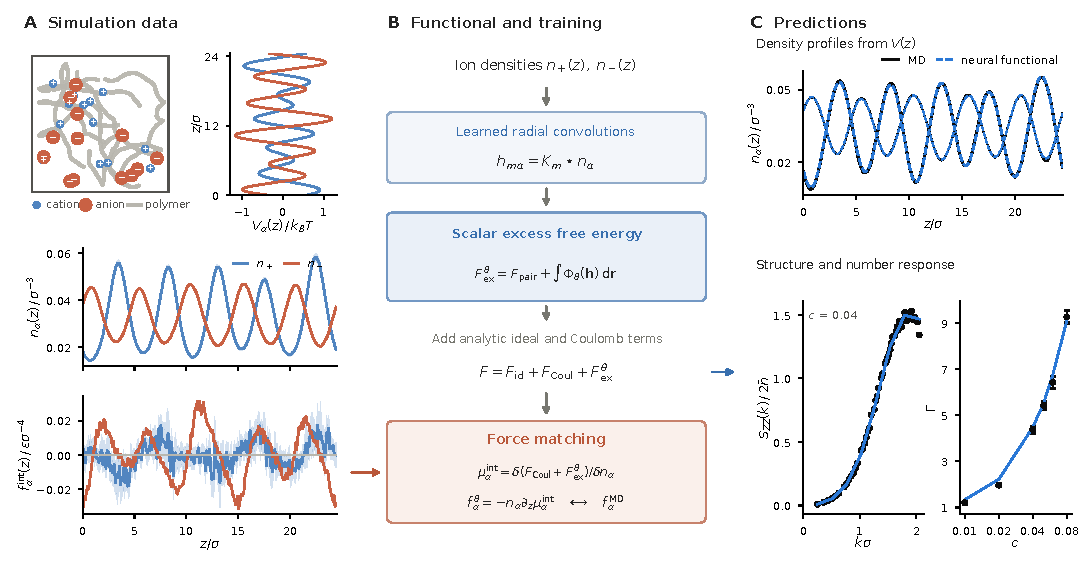
\includegraphics[width=\textwidth]{./fig1_schematic.pdf}
\caption{A learned density functional for the ions of a salt-doped polymer melt. (\textit{A}) Molecular dynamics under a planar external potential provides ion densities $n_\pm(z)$ and internal force densities $f^{\rm int}_\pm(z)$. (\textit{B}) Parameterize the excess free energy, which is trained by matching internal force densities to MD, where the ideal-gas and Coulomb contributions are included analytically. (\textit{C}) Predicted density profiles for a held-out run, bulk charge structure, and number response at the smallest nonzero wave number, compared with MD.}
\label{fig:model}
\end{figure*}


In this paper, we construct a neural functional for the ions of a coarse-grained salt-doped polymer melt \cite{tsamopoulos2024ion} (Fig.~\ref{fig:model}). The Coulomb interaction is kept analytically, and the remaining correlations are represented by a scalar functional of the cation and anion densities alone. This learned part is built from radial convolution kernels and a pointwise neural network, both defined in continuous space rather than on a grid. The chemical potentials are functional derivatives of the same scalar free-energy functional, so free-energy differences between density profiles do not depend on the integration path. The functional is invariant under all translations, rotations, and reflections. Therefore, the total internal force and torque vanish, as the Noether identities require \cite{hermann2021noether}. Because the Coulomb term is explicit and the learned kernels are short ranged, the small-wavenumber charge correlations satisfy the perfect-screening sum rules \cite{stillinger1968general} in stable, noncritical bulk states. Since no parameter refers to a grid or a box size, the trained functional can be evaluated in domains of other sizes and geometries.
 

We train this functional by matching species-resolved internal force densities measured in canonical molecular dynamics under static planar external potentials. The first Yvon--Born--Green equation connects these force densities to gradients of the interaction chemical potentials generated by the functional. This force-based supervision differs from fitting bulk pair correlations \cite{dijkman2025learning} or enforcing local chemical-potential balance \cite{sammuller2026determining,cheng2026equivariant}. The spatially constant chemical potentials drop out on taking the gradient, so the loss constrains the functional across inhomogeneous ionic environments without chemical-potential labels. Neither bulk structure factors nor the associated number susceptibility enters the force-matching loss, making them tests of the learned free-energy curvature beyond the fitted forces.

We study two electrostatic coupling strengths, with Bjerrum lengths of about $8$ and $30$ monomer diameters. At both, the functional trained on planar profiles predicts ionic structure in larger boxes and under external potentials that vary in two directions. The same functional describes density profiles at an untrained salt concentration and predicts bulk structure factors and the long-wavelength number response. Its nonlinear density dependence captures concentration-dependent effective ion correlations missed by a fixed quadratic pair closure, including the crossover from enhanced to suppressed long-wavelength number fluctuations at strong coupling. Compared with neural baselines trained under the same protocol, it reaches comparable or better accuracy while retaining its built-in structural identities.
% ---------------------------------------------------------------- Theory
\section*{A Structure-Preserving Neural Density Functional}

\subsection*{Free-energy formulation}
We consider a salt dissolved in a polymer melt. Treating the polymer implicitly, the ions are described by their number-density profiles $n_\alpha(\vr)$, with $\alpha\in\{+,-\}$, collected in $\vn=(n_+,n_-)$. Within classical density functional theory, these profiles are governed by the intrinsic free-energy functional
\begin{equation}
F[\vn]=\Fid[\vn]+\FC[\vn]+\Fex[\vn],
\label{eq:F}
\end{equation}
where
\(
\Fid[\vn]=k_BT\sum_\alpha\int \rmd\vr\,n_\alpha(\vr)\big[\ln\!\big(\Lambda^3n_\alpha(\vr)\big)-1\big]
\)
is the ideal-gas part, with thermal energy $k_BT$ and thermal wavelength $\Lambda$, and
\(
\FC[\vn]=\frac12\iint \rmd\vr\,\rmd\vr'\,\frac{\rho_Z(\vr)\rho_Z(\vr')}{4\pi\varepsilon_0\varepsilon_r|\vr-\vr'|}
\)
is the Coulomb mean-field energy of the charge density $\rho_Z(\vr)=\sum_\alpha e_\alpha n_\alpha(\vr)$. The ionic charges are $e_\alpha=z_\alpha e$, with valences $z_\pm=\pm1$ and elementary charge $e$. $\varepsilon_0$ is the vacuum permittivity and $\varepsilon_r$ the uniform relative permittivity of the medium. The excess part $\Fex[\vn]$ contains all correlations beyond the ideal gas and the Coulomb mean field and is the unknown component of the theory. With the polymer integrated out, $F$ is the intrinsic free energy of the ions in a melt that stays in equilibrium with their densities, so the response of the chains to the ions is part of $\Fex$. The functional therefore refers to one host state and coupling strength, here the melt of 30-bead chains at $k_BT=\epsilon$ and zero pressure at a given $\varepsilon_r$, and to the salt concentrations covered by the training data, 0.01 to 0.08 ion pairs per monomer, over which the melt volume adjusts to the salt content.

In external potentials $V_\alpha(\vr)$, the equilibrium profiles minimize $F+\sum_\alpha\int\rmd\vr\,V_\alpha n_\alpha$ at fixed particle numbers, which gives the Euler--Lagrange equations
\begin{equation}
k_BT\ln\!\big[\Lambda^3 n_\alpha(\vr)\big]+e_\alpha\phi(\vr)+\mu^{\rm ex}_\alpha(\vr;[\vn])+V_\alpha(\vr)=\mu_\alpha .
\label{eq:EL}
\end{equation}
The first three terms are the functional derivatives of $\Fid$, $\FC$ and $\Fex$ respectively. The mean electrostatic potential $\phi$ satisfies Poisson's equation, $-\nabla^2\phi=\rho_Z/(\varepsilon_0\varepsilon_r)$, the excess chemical potential is $\mu^{\rm ex}_\alpha=\delta\Fex/\delta n_\alpha(\vr)$, and the chemical potentials $\mu_\alpha$ are the Lagrange multipliers that fix the particle numbers.
 
Taking the gradient of Eq.~\ref{eq:EL} and combining it with the equilibrium force balance, the first equation of the Yvon--Born--Green hierarchy (derivation in \siref, section S2.2), gives
\begin{equation}
\vf_\alpha(\vr)=-n_\alpha(\vr)\,\nabla\mu^{\rm int}_\alpha(\vr;[\vn]),
\qquad
\mu^{\rm int}_\alpha=e_\alpha\phi+\mu^{\rm ex}_\alpha,
\label{eq:YBG}
\end{equation}
where $\vf_\alpha(\vr)$ is the equilibrium internal force density exerted on ions of species $\alpha$ by the other ions and the polymer monomers, excluding the external force. Eq.~\ref{eq:YBG} therefore relates a quantity sampled directly from the interaction forces in molecular dynamics to the functional, without chemical-potential labels. Since only the gradient of $\mu^{\rm int}_\alpha$ enters, force matching determines $\Fex$ only up to terms linear in the particle numbers $N_\alpha=\int\rmd\vr\,n_\alpha$, which shift $\mu_\alpha$ by constants.

 


\subsection*{The neural functional}
We parameterize the excess free energy as
\begin{align}
F^\theta_{\rm ex}[\vn]={}&
\frac12\sum_{\alpha\beta}\iint \rmd\vr\,\rmd\vr'\,
n_\alpha(\vr)\,u_{\alpha\beta}(|\vr-\vr'|)\,n_\beta(\vr')
\nonumber\\
&+\int \rmd\vr\,\Phi_\theta\big(\mathbf h(\vr)\big),
\label{eq:Fex}
\end{align}
where $\alpha,\beta$ denotes the species, $u_{\alpha\beta}=u_{\beta\alpha}$ are radial pair kernels and the neural network $\Phi_\theta$ is evaluated pointwise on the vector $\mathbf h(\vr)$ of weighted densities of both ionic species,
\[
h_{m\alpha}(\vr)=(K_m\star n_\alpha)(\vr).
\]
Here $\star$ denotes convolution, and the learned radial kernels $K_m$ probe the density profiles over multiple length scales. The first term is quadratic in the densities, with density-independent kernels while the second term makes the effective correlations depend nonlinearly on the surrounding densities. Because the kernels are continuous functions of distance and $\Phi_\theta$ acts pointwise, the functional is defined in continuous space: its parameters refer to no grid or box, and a discretization enters only when it is evaluated. The trainable parameters $\theta$ comprise the weights and biases of $\Phi_\theta$, the parameters defining the radial kernels $K_m$, and the coefficients defining the pair kernels $u_{\alpha\beta}$.
 
\subsection*{Properties of the neural functional}
With the excess part of Eq.~\ref{eq:Fex}, the functional $F$ of Eq.~\ref{eq:F} has the following properties by construction (proofs in \siref, section S1).
 
First, because the network represents the scalar $\Fex$ rather than the excess chemical potentials, the relation $\mu^{\rm ex}_\alpha=\delta\Fex/\delta n_\alpha$ holds exactly. The Hessian of $\Fex$, which gives the pair direct correlation functions, is therefore symmetric, and excess free-energy differences between density profiles do not depend on the integration path.
 
Second, $F$ is invariant under translations, rotations, and reflections, because all kernels are radial and $\Phi_\theta$ acts pointwise. Since the internal force densities of Eq.~\ref{eq:YBG} derive from this invariant scalar functional, Noether's theorem turns the invariance into global identities \cite{hermann2021noether}: for any admissible density profile, the total internal force and torque vanish after integration over space and summation over species.
 
Third, the functional satisfies the perfect-screening sum rules in stable, noncritical homogeneous bulk states. The explicit Coulomb term fixes the small-wavenumber charge response, while the short-ranged learned contribution has a finite limit as $k\to0$. For an electroneutral monovalent electrolyte, this gives
\begin{equation}
\frac{S_{ZZ}(k)}{2\nb}
=\frac{k^2}{\kappa_D^2}+O(k^4),
\qquad
\kappa_D^2=8\pi l_B\nb,
\label{eq:SL}
\end{equation}
where $S_{ZZ}(k)$ is the charge structure factor per unit volume, $\nb=\nb_+=\nb_-$ is the salt number density, $\kappa_D$ is the Debye wavenumber, and $l_B=e^2/(4\pi\varepsilon_0\varepsilon_r k_BT)$ is the Bjerrum length. The vanishing constant term and the $k^2$ coefficient encode the electroneutrality and Stillinger--Lovett second-moment conditions, respectively \cite{stillinger1968general}.
 
\subsection*{Training by force matching}
We train $F^\theta_{\rm ex}$ by matching Eq.~\ref{eq:YBG} to ion-density and internal force-density profiles from canonical molecular dynamics under static external potentials. For each run $r$, we evaluate the right-hand side of Eq.~\ref{eq:YBG} with $F^\theta_{\rm ex}$ on the sampled density profiles to obtain $\vf^\theta_{r\alpha}$. For the planar profiles used here, we denote the force-density residual along $z$ in bin $i$ by $\Delta_{r\alpha i}=f^{\rm MD}_{r\alpha}(z_i)-f^\theta_{r\alpha}(z_i)$. The parameters minimize the weighted squared residuals and the weighted squared Fourier amplitudes of the residuals,
\begin{equation}
\begin{aligned}
\mathcal L(\theta)={}&\sum_{r\alpha}\sum_{i=1}^{N_r}w_{r\alpha i}\,\Delta_{r\alpha i}^2\\
&+\sum_{r\alpha}\bar w_{r\alpha}\sum_{m=1}^{\lfloor N_r/2\rfloor}
\frac{2}{N_r}\,\frac{|\widehat\Delta_{r\alpha}(k_m)|^2}{(k_m\sigma)^2},
\end{aligned}
\label{eq:loss}
\end{equation}
where $N_r$ is the number of spatial bins and $\widehat{\Delta}_{r\alpha}(k_m)$ is the unnormalized discrete Fourier transform of the residual at wavenumber $k_m=2\pi m/L_r$, with box length $L_r$.

The first term weights each bin by
\(
w_{r\alpha i}=\frac{1}{s_{r\alpha i}^2+\bar s_{r\alpha}^2},
\)
where $s_{r\alpha i}$ is the MD standard error and $\bar s_{r\alpha}=\operatorname{median}_i s_{r\alpha i}$. These weights favor bins with small uncertainty, and the median floor $\bar s_{r\alpha}$ prevents bins with very small error bars from dominating the fit. The second term controls long-wavelength errors in the excess chemical potential. By Eq.~\ref{eq:YBG}, an error in $\mu^{\rm ex}_\alpha$ at wavenumber $k$ produces a force error that scales with $k$, so the first term penalizes such errors only weakly at small $k$. Dividing the squared Fourier amplitudes by $(k_m\sigma)^2$ compensates for this suppression. Because the Fourier amplitudes are not resolved by bin, each run enters this term with the mean of its bin weights, $\bar w_{r\alpha}=N_r^{-1}\sum_i w_{r\alpha i}$. 
% ---------------------------------------------------------------- Results
\section*{Results}

\begin{figure*}[tbhp]
\centering
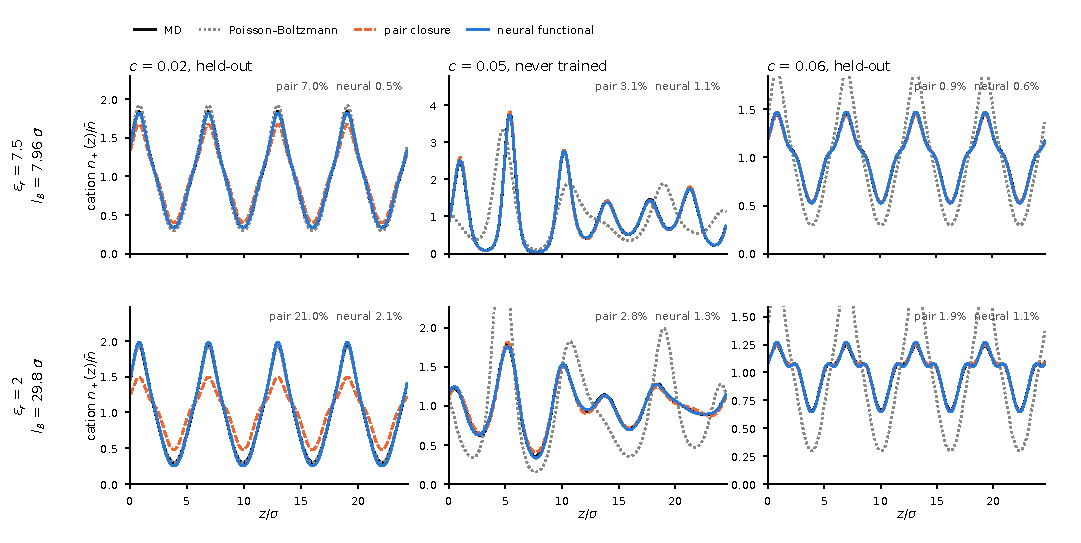
\includegraphics[width=\textwidth]{fig2.pdf}
\caption{Density profiles predicted for runs excluded from parameter fitting, at two coupling strengths. Top row: $\varepsilon_r=7.5$ ($l_B=7.96\sigma$); bottom row: $\varepsilon_r=2$ ($l_B=29.8\sigma$). Columns: a train of neutral Gaussian wells at $c=0.02$, the strongest well at the untrained concentration $c=0.05$, and a train of Gaussian wells at $c=0.06$. Cation densities relative to the mean; black curves and bands show MD averages and $\pm2$ standard errors estimated from eight blocks. Poisson--Boltzmann theory (dotted), the pair closure (dashed) and the neural functional (solid) are obtained by solving the canonical Euler--Lagrange equation under the applied potential. Numbers give the relative $L_2$ error of each profile, averaged over cations and anions.}
\label{fig:response}
\end{figure*}


\subsection*{Density profiles at held-out and untrained states}
We apply the method to a coarse-grained model of a salt-doped polymer melt \cite{tsamopoulos2024ion}. The melt contains 400 bead--spring chains, each comprising 30 monomers of diameter $\sigma$. The cation and anion diameters are $0.4\sigma$ and $1.6\sigma$, respectively, and both species are solvated by the monomers. The interaction potentials and model parameters are specified in \siref, section S2.1. We study two coupling strengths: at a dielectric constant of $\varepsilon_r=7.5$, the Bjerrum length is $l_B=7.96\sigma$; at $\varepsilon_r=2$, it is $l_B=29.8\sigma$, nearly four times as large. At each dielectric constant, we simulate five salt concentrations, $c=0.01, 0.02, 0.04, 0.06$, and $0.08$ cations per monomer, under static planar potentials $V_\alpha(z)$ acting on the ions. These potentials include superpositions of Fourier modes, trains of Gaussian wells, and modes with wavelengths equal to the box length, with amplitudes of up to a few $k_BT$. From approximately 100 runs at each dielectric constant, we hold out four at each concentration for testing. The test set consists of these 20 held-out runs and 22 additional runs at $c=0.05$, a concentration excluded from training.

We test the learned functional by solving Eq.~\ref{eq:EL} to predict equilibrium density profiles for the held-out runs (Fig.~\ref{fig:response}). We compare with two reference functionals. Poisson--Boltzmann theory is the mean-field limit $\Fex=0$. The pair closure serves as a quadratic reference: it keeps only the first term of Eq.~\ref{eq:Fex}, with density-independent kernels fitted to the same training data. Across all test runs, the mean relative $L_2$ errors of the neural functional are $1.2\%$ at $\varepsilon_r=7.5$ and $2.0\%$ at $\varepsilon_r=2$, compared with $3.0\%$ and $5.7\%$ for the pair closure and 25\% and 23\% for Poisson--Boltzmann theory. At the untrained concentration $c=0.05$, the mean relative $L_2$ errors are $0.85\%$ and $0.98\%$, respectively.
The advantage over the pair closure lies in describing several concentrations with one functional rather than in the accuracy at a single state. At $\varepsilon_r=7.5$, a pair closure fitted at $c=0.04$ alone yields profile errors of $1.9\%$ at that concentration, against $1.0\%$ for the neural functional (\siref, section S3.1). The effective correlations therefore depend on concentration, which we analyze below.

\subsection*{Transfer to larger boxes and nonplanar fields}
Because its parameters refer to no grid or box, the trained functional can be evaluated in larger domains without changing its parameters. We test transfer to a box twice the training length using an aperiodic potential containing a mode at half the smallest training wavenumber (Fig.~\ref{fig:generalization}\textit{A}). At both dielectric constants, the profile errors are 0.8\% to 1.6\%, against 2.4\% to 6.2\% for the pair closure. In a box four times the training length, a single mode at a quarter of the smallest training wavenumber gives profile errors of 0.5\% to 1.3\%, with driven amplitudes 6\% to 14\% below MD, against 0.8\% to 2.5\% and 11\% to 25\% for the pair closure (\siref, section S2.2).

The training profiles vary only along one direction, but the functional is defined for general three-dimensional densities. We therefore apply six potentials that vary in $x$ and $y$ at $c=0.04$: four periodic ones, including square lattices of rods and wavevectors oblique to the box axes, and two aperiodic ones that combine oblique plane waves with irregularly placed Gaussian wells and barriers (Fig.~\ref{fig:generalization} \textit{B} and \textit{C}). For the aperiodic potentials, the relative profile errors of the predicted density maps are 1.8--3.1\%, at the level of the MD noise of 1.7--3.0\%, against 3.6--5.5\% for the pair closure and 31--62\% for Poisson--Boltzmann theory (\siref, section S4.1).


\begin{figure*}[!t]
\centering
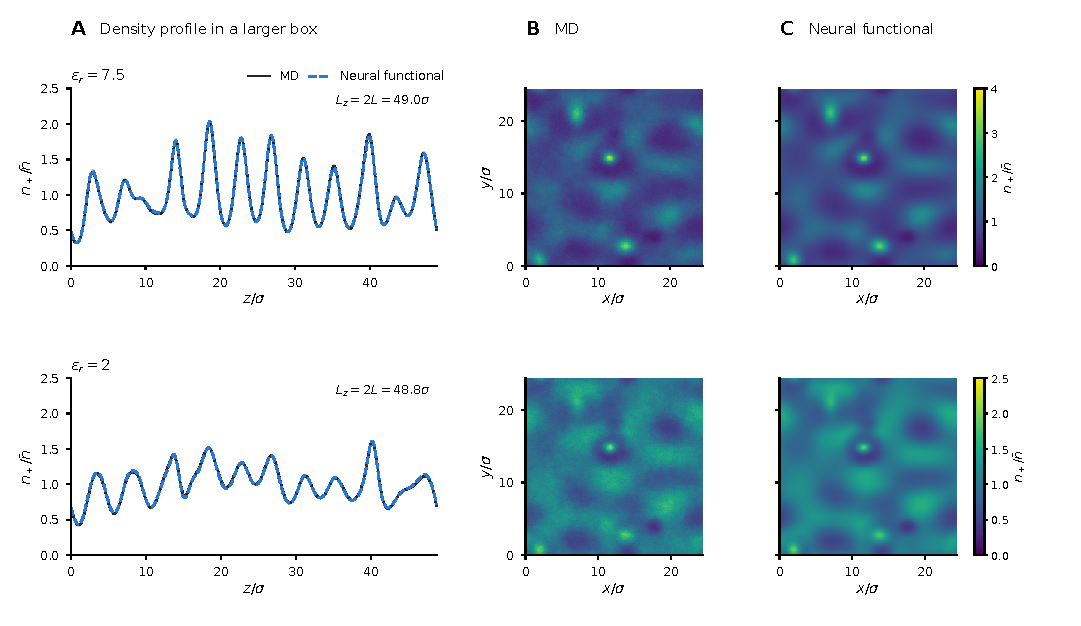
\includegraphics[width=\textwidth]{generalization.pdf}
\caption{Generalization to larger boxes and nonplanar density fields at $c=0.04$. Rows correspond to $\varepsilon_r=7.5$ and 2. (\textit{A}) Cation density profiles in a box twice the training length under an aperiodic potential. Black curves and gray bands show MD averages and $\pm2$ archived standard errors; blue dashed curves show the neural-functional prediction. (\textit{B}, \textit{C}) MD and predicted cation densities under an aperiodic two-dimensional potential of oblique plane waves and irregularly placed Gaussian wells and barriers, using a shared color scale within each row. All predictions use parameters trained on planar profiles in the original box.}
\label{fig:generalization}
\end{figure*}


\begin{figure}[tbhp]
\centering
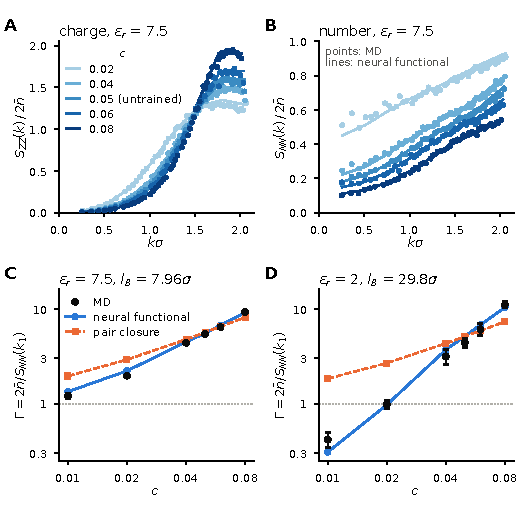
\includegraphics[width=\linewidth]{fig3.pdf}
\caption{Bulk structure and long-wavelength number response. (\textit{A}, \textit{B}) Normalized charge and number structure factors at $\varepsilon_r=7.5$ and $c=0.02$ to $0.08$. Points show zero-field MD results averaged over $k$-shells; curves show predictions from Eq.~\ref{eq:OZ}. (\textit{C}, \textit{D}) Finite-wavenumber response factor $\Gamma(k_1)=2\nb/S_{NN}(k_1)$ at $\varepsilon_r=7.5$ and $2$. Solid curves show the neural functional and dashed curves the pair closure. The dotted line marks the ideal value $\Gamma=1$. Neither quantity enters the force-matching loss.}
\label{fig:structure}
\end{figure}

\subsection*{Bulk structure and long-wavelength response}
In a uniform bulk state, density fluctuations are determined by the Hessian of the free energy, a quantity not used in training. We define the Fourier-space excess kernel as
\[
W_{\alpha\beta}(k)
=\int\rmd\vr\,e^{-i\mathbf k\cdot\vr}\,
\frac{\delta^2\Fex}
{\delta n_\alpha(\vr)\,\delta n_\beta(\mathbf 0)}
\bigg|_{\vn=(\nb_+,\nb_-)}.
\]
Including the ideal-gas and Coulomb contributions, the Ornstein--Zernike relation gives
\begin{equation}
S(k)^{-1}
=\bar N^{-1}
+\frac{4\pi l_B}{k^2}\,\vz\vz^{\T}
+\frac{W(k)}{k_BT},
\label{eq:OZ}
\end{equation}
where $S_{\alpha\beta}(k)$ are the partial structure factors per unit volume. Here $\bar N={\rm diag}(\nb_+,\nb_-)$ contains the bulk densities, and $\vz=(1,-1)^{\T}$ is the valence vector.

Projecting $S(k)$ onto the charge and number-density channels gives
\[
S_{ZZ}(k)=\vz^{\T}S(k)\vz,
\qquad
S_{NN}(k)=\mathbf q^{\T}S(k)\mathbf q,
\]
where $\mathbf q=(1,1)^{\T}$.
At $\varepsilon_r=7.5$ and $c=0.02-0.08$, the neural functional reproduces the zero-field MD charge and number structure factors with relative root-mean-square errors of $2.7-4.1\%$ and $2.4-3.6\%$, respectively, over $0.25\leq k\sigma\leq2.1$ (Fig.~\ref{fig:structure}\textit{A} and \textit{B}).

We quantify the long-wavelength number response by $\Gamma(k)=2\nb/S_{NN}(k)$, which equals 1 for an ideal solution. In the finite simulation box, we report $\Gamma(k_1)$ at the smallest wavenumber $k_1=2\pi/L$. At $\varepsilon_r=2$, the MD estimate rises from $0.42\pm0.07$ at $c=0.01$ to $11.1\pm0.8$ at $c=0.08$ (Fig.~\ref{fig:structure}\textit{D}), describing enhanced number fluctuations at low concentration and suppressed fluctuations at high concentration. The neural functional reproduces this concentration dependence at both dielectric constants, whereas the pair closure gives $\Gamma(k_1)>1$ at all concentrations at $\varepsilon_r=2$ and misses the enhanced fluctuations. 

To identify which correlations contribute most of the concentration dependence of $\Gamma(k_1)$, including the crossover at $\varepsilon_r=2$, we return to Eq.~\ref{eq:OZ}. At small wavenumbers, its Coulomb term strongly suppresses charge fluctuations, so the number channel nearly decouples and
\begin{equation}
\Gamma(k_1)\simeq1+\frac{\nb}{2k_BT}\,\mathbf q^{\T}W(k_1)\mathbf q,
\label{eq:Gamma}
\end{equation}
where $\mathbf q^{\T}W\mathbf q=W_{++}+W_{--}+2W_{+-}$ is the excess kernel in the number channel. Number fluctuations are therefore enhanced when $\mathbf q^{\T}W\mathbf q<0$, and suppressed when $\mathbf q^{\T}W\mathbf q>0$. A fixed quadratic pair closure has a density-independent $W(k)$, so $\Gamma(k_1)-1$ keeps its sign at all concentrations. The neural term instead allows $W(k)$ to vary with the surrounding ion densities. The number-channel kernel inferred from zero-field MD changes sign with concentration at $\varepsilon_r=2$, and the neural functional reproduces its concentration dependence at both dielectric constants (Fig.~\ref{fig:manybody}).
 
 
\begin{figure}[tbhp]
\centering
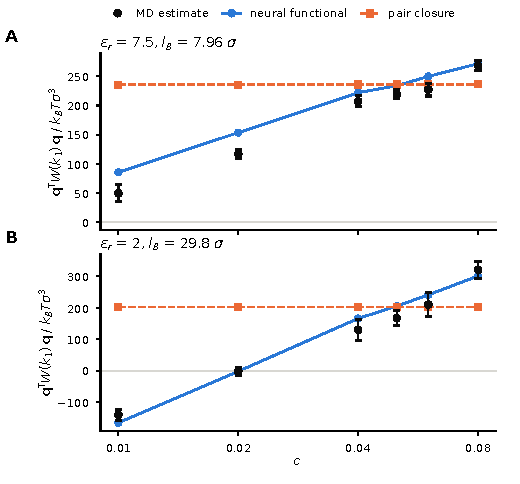
\includegraphics[width=\linewidth]{fig4.pdf}
\caption{Concentration dependence of effective correlations. Combined correlation kernel $\mathbf q^{\T}W(k_1)\mathbf q$ versus concentration at $\varepsilon_r=7.5$ (\textit{A}) and 2 (\textit{B}). Points show estimates from zero-field MD (\siref, section S3.2); solid curves show the neural functional and dashed curves the pair closure.}
\label{fig:manybody}
\end{figure}


\subsection*{Comparison with other learned functionals}
We next compare our functional with existing learned functionals: the one-body network of refs.~\cite{sammuller2023neural,bui2025learning}, which predicts excess chemical potentials directly from local density profiles; the convolutional free energy of ref.~\cite{dijkman2025learning}, which maps the whole planar profile to a free energy; and the lattice free energy of ref.~\cite{cheng2026equivariant}, which represents the excess free energy through Cartesian moments of local density environments. 
As discussed above, these models differ in the structural properties guaranteed by their original formulations (Table~\ref{tab:architectures}). Here, we further test numerically whether these differences also affect predictive performance. To this end, we adapt each architecture to the force-matching protocol of our functional and train it on the same data and splits.
 
The comparison uses two systems. The first is the truncated Lennard-Jones fluid of ref.~\cite{cheng2026equivariant}, a one-component fluid without charges as in refs.~\cite{sammuller2023neural,dijkman2025learning,cheng2026equivariant}. The second is the present ionic system, on which all forms include the same analytic Coulomb term. Table~\ref{tab:compare} reports the mean relative $L_2$ errors of the density profiles that each form predicts by solving the Euler--Lagrange equation.

To assess how strongly each method depends on the amount of training data, we compare them at two training-set sizes: the full training set and about a quarter of it. We expect our functional to need less data than the baselines. Enforcing integrability and symmetry restricts the space of admissible functionals, so fewer training data are needed to determine the functional.

On the Lennard-Jones fluid at $T=1.5$ (\methodsref), our functional is the most accurate method at both sizes. Trained on all 74 training runs, it reaches a mean held-out profile error of $0.27\%$, compared with $0.64\%$ for the one-body network and $0.54\%$ for the lattice free energy. Trained on 20 of these runs, its error rises only to $0.30\%$. The error of the one-body network rises to $0.70\%$, and that of the lattice free energy grows by about half, to $0.80\%$. The convolutional free energy rarely reaches a converged solution. Trained on all runs, its Euler--Lagrange iteration converges for 7 of the 20 held-out runs and for none of the 21 runs at the untrained density. For runs that do not converge, we take the density at the last iteration before the solver stops. The resulting mean profile errors are $2.0\%$ with all training runs and $3.2\%$ with a quarter of them, seven to ten times ours. On this simple fluid, our functional is thus about twice as accurate as the best baseline at either training-set size.

The ions are a more demanding test, and every method has larger errors than on the Lennard-Jones fluid. With the full training set, the one-body network is nearly as accurate as our functional: its held-out profile errors are $1.75\%$ and $3.41\%$ at $\varepsilon_r=7.5$ and $2$, compared with $1.50\%$ and $3.11\%$ for ours. The two free-energy baselines are less accurate. The lattice free energy fails for 4 of the 42 test runs at $\varepsilon_r=7.5$ and for 10 at $\varepsilon_r=2$. In these runs its Euler--Lagrange iteration either does not converge or converges to an unphysical state in which the density collapses into a narrow spike. Over the remaining runs, its mean held-out profile errors are $2.97\%$ and $7.16\%$, about twice ours, and its bulk structure factors deviate from MD by up to 26\%. The convolutional free energy was trained here by force matching rather than by the pair-correlation matching of the original work. It converges for at most 5 of its 42 test runs, and its final iterates deviate from MD by $14\%$ and $15\%$.

The constraints pay off once the training set is reduced. With a quarter of the runs, our held-out profile errors change little: from $1.50\%$ to $1.55\%$ at $\varepsilon_r=7.5$, and from $3.11\%$ to $3.56\%$ at $\varepsilon_r=2$. The errors of the one-body network grow by 60--70\%, to $3.00\%$ and $5.55\%$, and 3 of its 20 held-out solutions at $\varepsilon_r=7.5$ no longer converge (\siref, section S4.3). Its errors are then 1.6--1.9 times ours, compared with 1.1--1.2 times with the full training set.
 
In both systems, our functional is the most accurate method with the full training set and loses the least accuracy when three quarters of the training data are removed. This is consistent with the constraints reducing what must be learned from data. We agree that the baselines may become more competitive with larger training sets. With only a quarter of the runs, however, our functional is already more accurate than every baseline trained on all of them for the Lennard-Jones fluid, and about as accurate as the one-body network trained on all of them for the ions.
 
The structural checks on the MD profiles show the differences of Table~\ref{tab:architectures} in the adapted implementations (Table~\ref{tab:compare}). The one-body network has net-force errors of up to 14\%, Jacobian asymmetries of up to 55\% and path-dependent free-energy differences of up to 1\%. The two free-energy baselines have symmetric Hessians, but their net-force errors reach $7\times10^{-4}$ and 6\%, since the Noether identity is not guaranteed without invariance under continuous translations. Our functional has a maximum net-force error of $2\times10^{-6}$, with a symmetric Hessian and path-independent free-energy differences to numerical precision. On the same profiles resampled to $0.05\sigma$ and $0.2\sigma$ grids, its chemical potentials change by less than $10^{-4}$, those of the one-body network and the lattice free energy by 62--79\%, and the convolutional free energy cannot be evaluated (\siref, section S4.3).
 
\begin{table*}[tb]
\centering
\caption{Profile errors and structural checks of the adapted baselines, our functional and the pair closure. Profile errors are mean relative $L_2$ errors (\%) as in Fig.~\ref{fig:response}; the statistical errors of the MD profiles are about 1\%. ``Quarter'' denotes training on a quarter of the runs. Means exclude failed solutions (footnotes), except for the convolutional free energy, whose entries are errors of the final iterates. Structural checks give maxima on the MD profiles of the ions: relative net internal force, Hessian asymmetry and path dependence of the free energy (\siref, section S4.3).}
\label{tab:compare}
\small
\setlength{\tabcolsep}{3pt}\begin{tabular}{lcccccccccccc}
 & & \multicolumn{2}{c}{Lennard-Jones} & \multicolumn{6}{c}{Ions} & \multicolumn{3}{c}{Structural checks}\\
\cmidrule(lr){3-4}\cmidrule(lr){5-10}\cmidrule(lr){11-13}
 & & & & \multicolumn{2}{c}{held-out} & \multicolumn{2}{c}{$c=0.05$} & \multicolumn{2}{c}{quarter} & & & \\
\cmidrule(lr){5-6}\cmidrule(lr){7-8}\cmidrule(lr){9-10}
Form & Parameters & all & quarter & $\varepsilon_r=7.5$ & 2 & 7.5 & 2 & 7.5 & 2 & Force & Hessian & Path\\
\midrule
Neural functional (this work) & 19{,}641 & 0.27 & 0.30 & 1.50 & 3.11 & 0.85 & 0.98 & 1.55 & 3.56 & $2\times10^{-6}$ & $3\times10^{-16}$ & $2\times10^{-12}$\\
One-body network~\cite{sammuller2023neural,bui2025learning}$^{a}$ & 32{,}514 & 0.64 & 0.70 & 1.75 & 3.41 & 1.01 & 0.85 & 3.00 & 5.55 & 0.14 & 0.55 & 0.009\\
Lattice free energy~\cite{cheng2026equivariant}$^{b}$ & 23{,}828 & 0.54 & 0.80 & 2.97 & 7.16 & 2.06 & 2.72 & 4.53 & 6.31 & $7\times10^{-4}$ & $2\times10^{-16}$ & $7\times10^{-8}$\\
Convolutional free energy~\cite{dijkman2025learning}$^{c}$ & 24{,}321 & 2.03 & 3.20 & 13.8 & 15.1 & 16.1 & 16.2 & -- & -- & 0.06 & $10^{-16}$ & $10^{-15}$\\
Pair closure & 1{,}336 & 12.1 & -- & 4.21 & 8.78 & 1.91 & 2.58 & -- & -- & \multicolumn{3}{c}{exact}\\
\bottomrule
\end{tabular}\par\smallskip
\tablenote{$^{a}$With a quarter of the runs, it fails to converge for 3 of the 20 held-out ion runs at $\varepsilon_r=7.5$ and for 1 of the 41 Lennard-Jones runs. $^{b}$Trained on all runs, it fails for 4 of the 42 ion test runs at $\varepsilon_r=7.5$ (3 not converged, 1 collapsed) and for 10 at $\varepsilon_r=2$ (6 not converged, 4 collapsed); trained on a quarter of the runs, it fails for 2 and 7 of the 20 held-out runs at $\varepsilon_r=7.5$ and 2, respectively. $^{c}$Trained on all runs, it converges for 5 of the 42 ion test runs at $\varepsilon_r=7.5$, for none at $\varepsilon_r=2$, and for 7 of the 41 Lennard-Jones runs; it is not trained on a quarter of the ion runs.}
\end{table*}
% ---------------------------------------------------------------- Discussion
\section*{Discussion}
We construct a neural density functional for the ions of a salt-doped polymer melt that satisfies all the structural properties in Table~\ref{tab:architectures} by construction. Previous neural functionals, developed mostly for simple fluids, each guarantee only some of them.
Trained only on planar force densities, the same functional predicts ionic structure in larger boxes and in fields that vary in two directions, describes an untrained salt concentration, and recovers bulk structure factors and the long-wavelength number response. This is an important step toward carrying the accuracy of MD, currently limited to small systems, over to larger and more complex ones.

A natural next step is application on transport problem. Although the functional describes equilibrium, it supplies the chemical potentials whose gradients drive ion fluxes in stochastic and dynamical density functional theories \cite{dean1996langevin,avni2022conductivity}. Combined with a validated mobility model, it could predict conductivity and salt diffusion that include the ion correlations learned here. We also plan to apply the functional at electrode interfaces, where its three-dimensional, grid-independent form can be used once the boundary conditions and the polymer environment are specified.
\matmethods{\subsection*{Molecular dynamics}
We simulate the coarse-grained model of Tsamopoulos and Wang \cite{tsamopoulos2024ion}: 400 chains of 30 beads joined by FENE bonds \cite{KremerGrest1990}, with 120 to 960 cation--anion pairs for $c=0.01$ to $0.08$. Both ions interact with the monomers through the solvation potential of Hall and coworkers \cite{shen2020ion}, of strength $4.33\,k_BT$ and range $5\sigma$. 
Electrostatics uses PPPM \cite{hockney2021computer} with dielectric constant 7.5 or 2. All runs use LAMMPS \cite{thompson2022lammps} with a Nos\'e--Hoover thermostat \cite{nose1984unified,hoover1985canonical} at $k_BT=\epsilon$ and a time step of $0.005\tau$. Each state point is equilibrated at zero pressure and then simulated at the mean volume(\siref, section S2.1).

\subsection*{External potentials and profiles}
The potentials $V_\pm(z)=V_N(z)\pm\psi(z)$ consist of a part $V_N$ that acts equally on both species and a part $\psi$ that acts with opposite signs, like an applied electrostatic potential. They belong to four families that cover different length scales: Fourier series with wavenumbers $k_m=2\pi m/L$ for $m=3$ to $6$, the same series with additional modes up to $m=20$, trains of Gaussian wells, and long-wavelength modes with $m=1$ and $2$.  Each run is equilibrated in the field for $6\times10^3$ to $4\times10^4\,\tau$ and then sampled for $3.7\times10^4$ to $2.0\times10^5\,\tau$, longer at higher concentration. Density and internal force density profiles are recorded on $0.1\sigma$ bins, with standard errors estimated from eight consecutive blocks of each trajectory.

\subsection*{Neural functional and training}
The pair kernels and the weighted densities in Eq.~\ref{eq:Fex} are built from six learned radial kernels $K_m(r)=B_m(r)[1+g_m(r)]$, where $B_m$ are normalized Gaussians of widths $0.25$ to $1\sigma$ and $g$ is a perceptron of $r$ with two hidden layers of 32 units and six outputs. The pair kernels are parameterized as $u_{\alpha\beta}(r)=\sum_m a_{\alpha\beta m}K_m(r)$, with learned coefficients $a_{\alpha\beta m}=a_{\beta\alpha m}$. $\Phi_\theta$ is a perceptron with two hidden layers of 128 units that acts on the 12 weighted densities. Both networks use softplus activations, and the functional has 19{,}641 parameters. We minimize the loss with AdamW \cite{LoshchilovHutter2019} (learning rate $10^{-3}$ with cosine decay, weight decay $10^{-5}$) for 4000 steps and keep the parameters with the lowest validation residual. 

\subsection*{Other learned functionals}
For the comparison in Table~\ref{tab:compare}, we adapt three published forms to the two ion species and the analytic Coulomb term and train them with the same data, splits and force-matching loss as our functional. The one-body network \cite{sammuller2023neural,bui2025learning} is a single perceptron with two hidden layers of 128 units that maps the densities of both species within $\pm3\sigma$ of a point to $\mu^{\rm ex}_+$ and $\mu^{\rm ex}_-$ at that point. The lattice free energy \cite{cheng2026equivariant} uses $O_h$-invariant products of Cartesian density moments on $0.5\sigma$ voxels. Moments are resolved by species, and invariants are formed within and across species. For planar profiles, the densities are averaged onto the voxels, the sums over lateral stencil offsets are evaluated exactly, and the free energy is averaged over the registrations of the lattice with the profile. The window is chosen by the validation residual, which favors $\pm3\sigma$ over $\pm6\sigma$, and the stencil radius is that of the original, $1.5\sigma$ (\siref, section S4.2). The convolutional free energy \cite{dijkman2025learning} passes the two densities, as input channels, through six periodic dilated convolutions (kernel 3, dilation 2, 16 to 64 channels), each followed by average pooling, and a linear read-out; all layers use softplus activations. The Lennard-Jones benchmark is the truncated and shifted fluid of ref.~\cite{cheng2026equivariant} ($r_c=2.5\sigma$, $T=1.5$) in a cubic box of side $24\sigma$. Training uses the densities $\rho\sigma^3=0.1$, $0.2, 0.4, 0.6$ and $0.7$, each with $22$ planar potentials, and the density $0.5$ is held out.}
\showmatmethods{}
\dataavail{\PaperDataAvailability}
\acknow{\PaperAcknowledgments}
\showacknow{}
\bibliography{references}
\end{document}
